\section{Event samples}
\label{sec:event-samples}

\subsection{Standard model MC samples}
\label{sec:sm-mc}
Monte Carlo (MC) samples reconstructed with CMSSW release 8\_0\_X (Summer16) are used for all processes. The SM samples are listed in Tables \ref{tab:ttbarMCsamples}, \ref{tab:qcdMCsamples}, \ref{tab:zjetsMCsamples}, and \ref{tab:wjetsMCsamples}. The cross sections listed correspond to next-to-next-to-leading-order (NNLO) calculations unless otherwise noted.  All samples use the PU25bx25 pileup scenario, which simulates a pileup distribution with an average of 25 interactions per bunch crossing and a 25 ns interval between bunches. The Monte Carlo samples are used to validate the data-driven background estimation methods.

\begin{table}[hp!]
\centering
\caption{SM \ttbar MC samples used in the analysis. The cross
  sections are calculated to NNLO. }
\label{tab:ttbarMCsamples}
{\footnotesize
\begin{tabular}{lcc}
\hline \hline
Dataset & $\sigma$ (pb) & $\int\mathbb{L}$ (fb$^{-1}$) \\
\hline
%TTJets\_TuneCUETP8M1\_13TeV-madgraphMLM-pythia8 & 831.76 & 12.34\\
TTJets\_SingleLeptFromT\_TuneCUETP8M1\_13TeV-madgraphMLM-pythia8 & 182.72 & 283.90\\
TTJets\_SingleLeptFromTbar\_TuneCUETP8M1\_13TeV-madgraphMLM-pythia8 & 182.72 & 326.48\\
TTJets\_DiLept\_TuneCUETP8M1\_13TeV-madgraphMLM-pythia8 & 88.34 & 346.25\\
TTJets\_HT-600to800\_TuneCUETP8M1\_13TeV-madgraphMLM-pythia8 & 2.734 & 5231.81\\
TTJets\_HT-800to1200\_TuneCUETP8M1\_13TeV-madgraphMLM-pythia8 & 1.121 & 9416.61\\
TTJets\_HT-1200to2500\_TuneCUETP8M1\_13TeV-madgraphMLM-pythia8 & 0.198 & 14819.34\\
TTJets\_HT-2500toInf\_TuneCUETP8M1\_13TeV-madgraphMLM-pythia8 & 0.002 & 221088.29\\
\hline \hline
\end{tabular}
}
\end{table}

\begin{table}[hp!]
\centering
\caption{SM QCD MC samples used in the analysis. All cross sections are calculated to LO.}
\label{tab:qcdMCsamples}
{\footnotesize
\begin{tabular}{lcc}
\hline \hline
Dataset & $\sigma$ (pb) & $\int\mathbb{L}$ (fb$^{-1}$) \\
\hline
QCD\_HT200to300\_TuneCUETP8M1\_13TeV-madgraphMLM-pythia8 & 1735000 & 0.03\\
QCD\_HT300to500\_TuneCUETP8M1\_13TeV-madgraphMLM-pythia8 & 366800 & 0.16\\
QCD\_HT500to700\_TuneCUETP8M1\_13TeV-madgraphMLM-pythia8 & 29370 & 1.95\\
QCD\_HT700to1000\_TuneCUETP8M1\_13TeV-madgraphMLM-pythia8 & 6524 & 6.68\\
QCD\_HT1000to1500\_TuneCUETP8M1\_13TeV-madgraphMLM-pythia8 & 1064 & 12.62\\
QCD\_HT1500to2000\_TuneCUETP8M1\_13TeV-madgraphMLM-pythia8 & 121.5 & 32.63\\
QCD\_HT2000toInf\_TuneCUETP8M1\_13TeV-madgraphMLM-pythia8 & 25.42 & 239.30\\
\hline \hline
\end{tabular}
}
\end{table}

\begin{table}[hp!]
\centering
\caption{SM $Z\rightarrow\nu\nu+$jets MC samples used in the analysis. The cross sections are calculated to NNLO. }
\label{tab:zjetsMCsamples}
{\footnotesize
\begin{tabular}{lcc}
\hline \hline
Dataset & $\sigma$ (pb) & $\int\mathbb{L}$ (fb$^{-1}$) \\
\hline
ZJetsToNuNu\_HT-100To200\_13TeV-madgraph & 344.8 & 54.13\\
ZJetsToNuNu\_HT-200To400\_13TeV-madgraph & 95.53 & 208.46\\
ZJetsToNuNu\_HT-400To600\_13TeV-madgraph & 13.20 & 77.30\\
ZJetsToNuNu\_HT-600To800\_13TeV-madgraph & 3.148 & 1795.26\\
ZJetsToNuNu\_HT-800To1200\_13TeV-madgraph & 1.451 & 1486.09\\
ZJetsToNuNu\_HT-1200To2500\_13TeV-madgraph & 0.355 & 1029.81\\
ZJetsToNuNu\_HT-2500ToInf\_13TeV-madgraph & 0.0085 & 47498.87\\
\hline \hline
\end{tabular}
}
\end{table}
\begin{table}[hp!]
\centering
\caption{SM $W\rightarrow\ell\nu+$jets MC samples used in the analysis. The cross sections are calculated to NNLO.}
\label{tab:wjetsMCsamples}
{\footnotesize
\begin{tabular}{lcc}
\hline \hline
Dataset & $\sigma$ (pb) & $\int\mathbb{L}$ (fb$^{-1}$) \\
\hline
WJetsToLNu\_HT-100To200\_TuneCUETP8M1\_13TeV-madgraphMLM-pythia8 & 1627.45 & 18.16\\
WJetsToLNu\_HT-200To400\_TuneCUETP8M1\_13TeV-madgraphMLM-pythia8 & 435.24 & 45.88\\
WJetsToLNu\_HT-400To600\_TuneCUETP8M1\_13TeV-madgraphMLM-pythia8 & 59.18 & 123.64\\
WJetsToLNu\_HT-600To800\_TuneCUETP8M1\_13TeV-madgraphMLM-pythia8 & 14.58 & 221.32\\
WJetsToLNu\_HT-800To1200\_TuneCUETP8M1\_13TeV-madgraphMLM-pythia8 & 6.66 & 1123.13\\
WJetsToLNu\_HT-1200To2500\_TuneCUETP8M1\_13TeV-madgraphMLM-pythia8 & 1.608 & 153.44\\
WJetsToLNu\_HT-2500ToInf\_TuneCUETP8M1\_13TeV-madgraphMLM-pythia8 & 0.039 & 6497.28\\
\hline \hline
\end{tabular}
}
\end{table}

\subsection{Signal models}
\label{sec:signal-models}

\begin{figure}[htbp!]
\centering
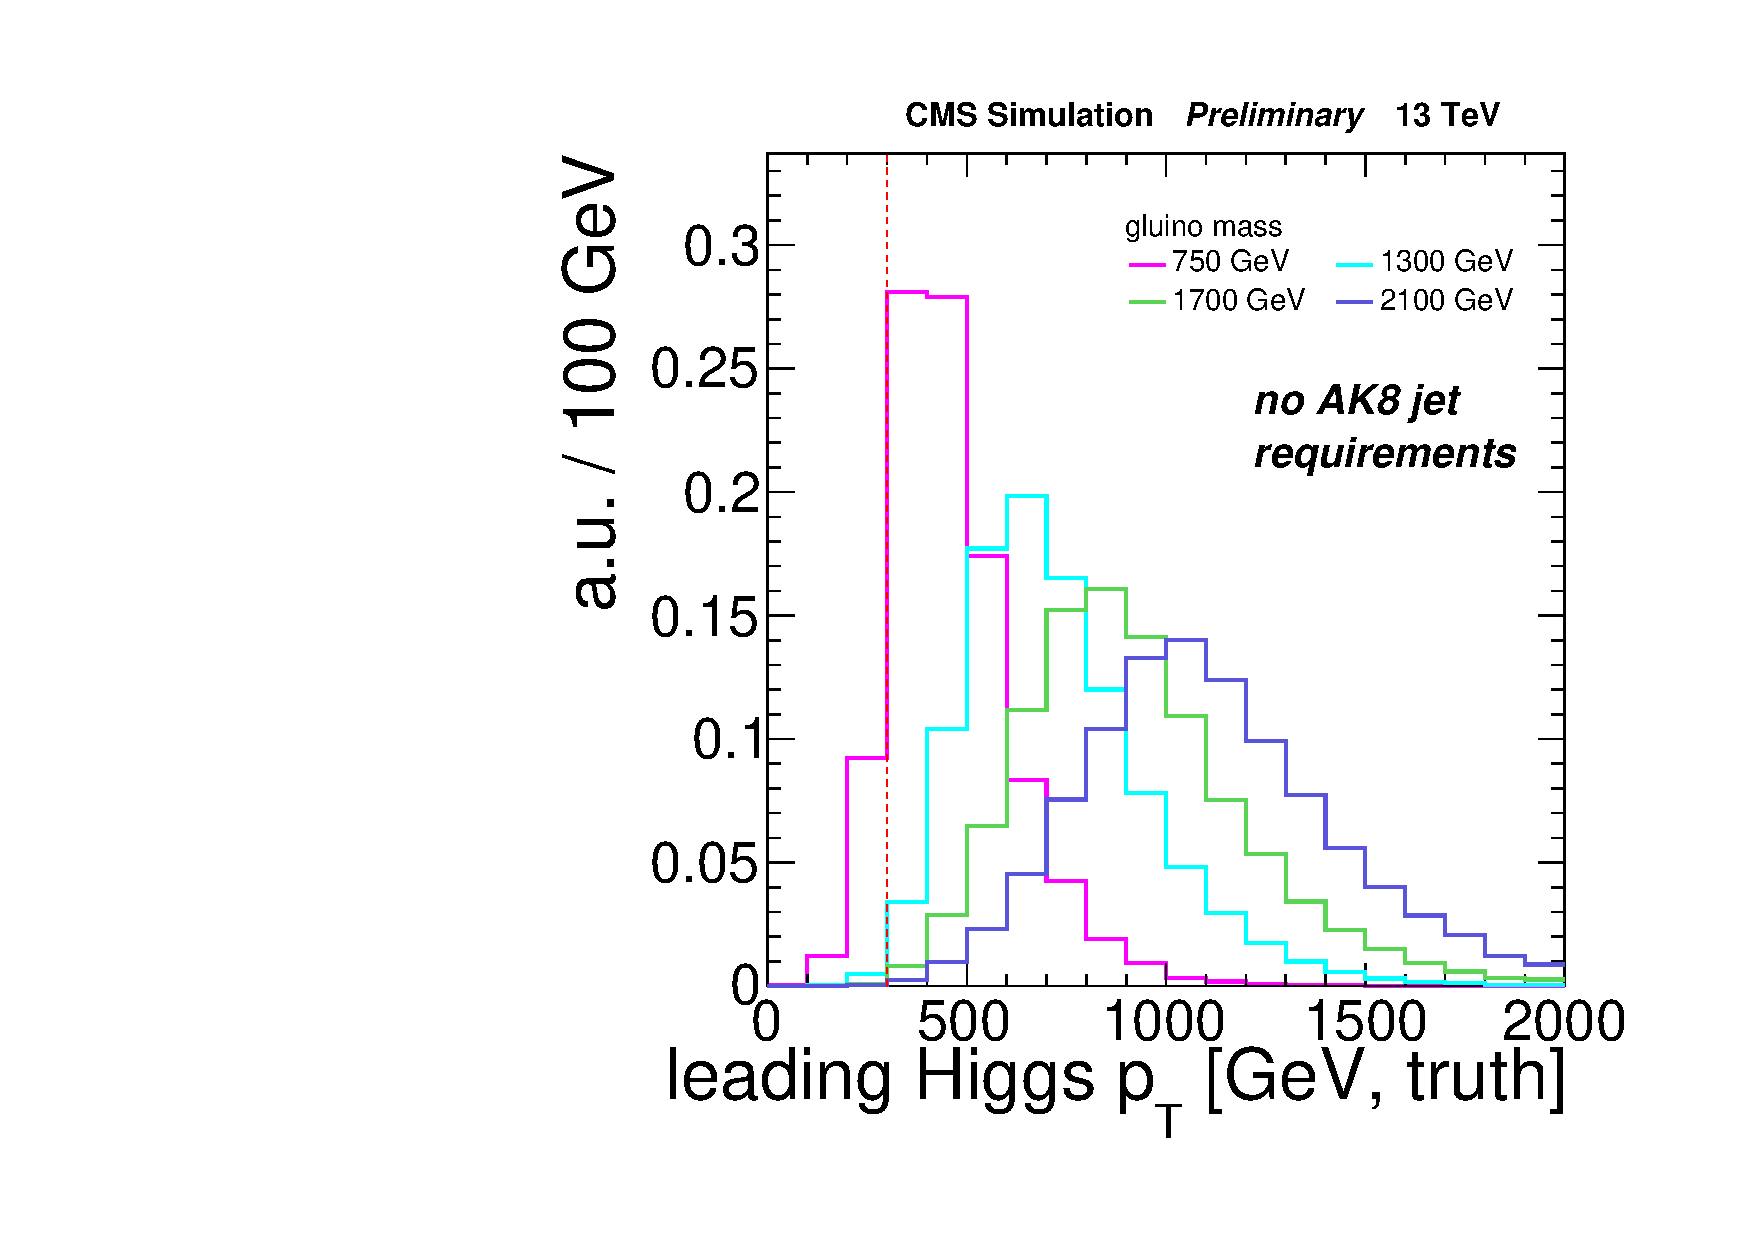
\includegraphics[width=0.45\linewidth]{figs/SUS17006/leadHiggsPt.pdf}
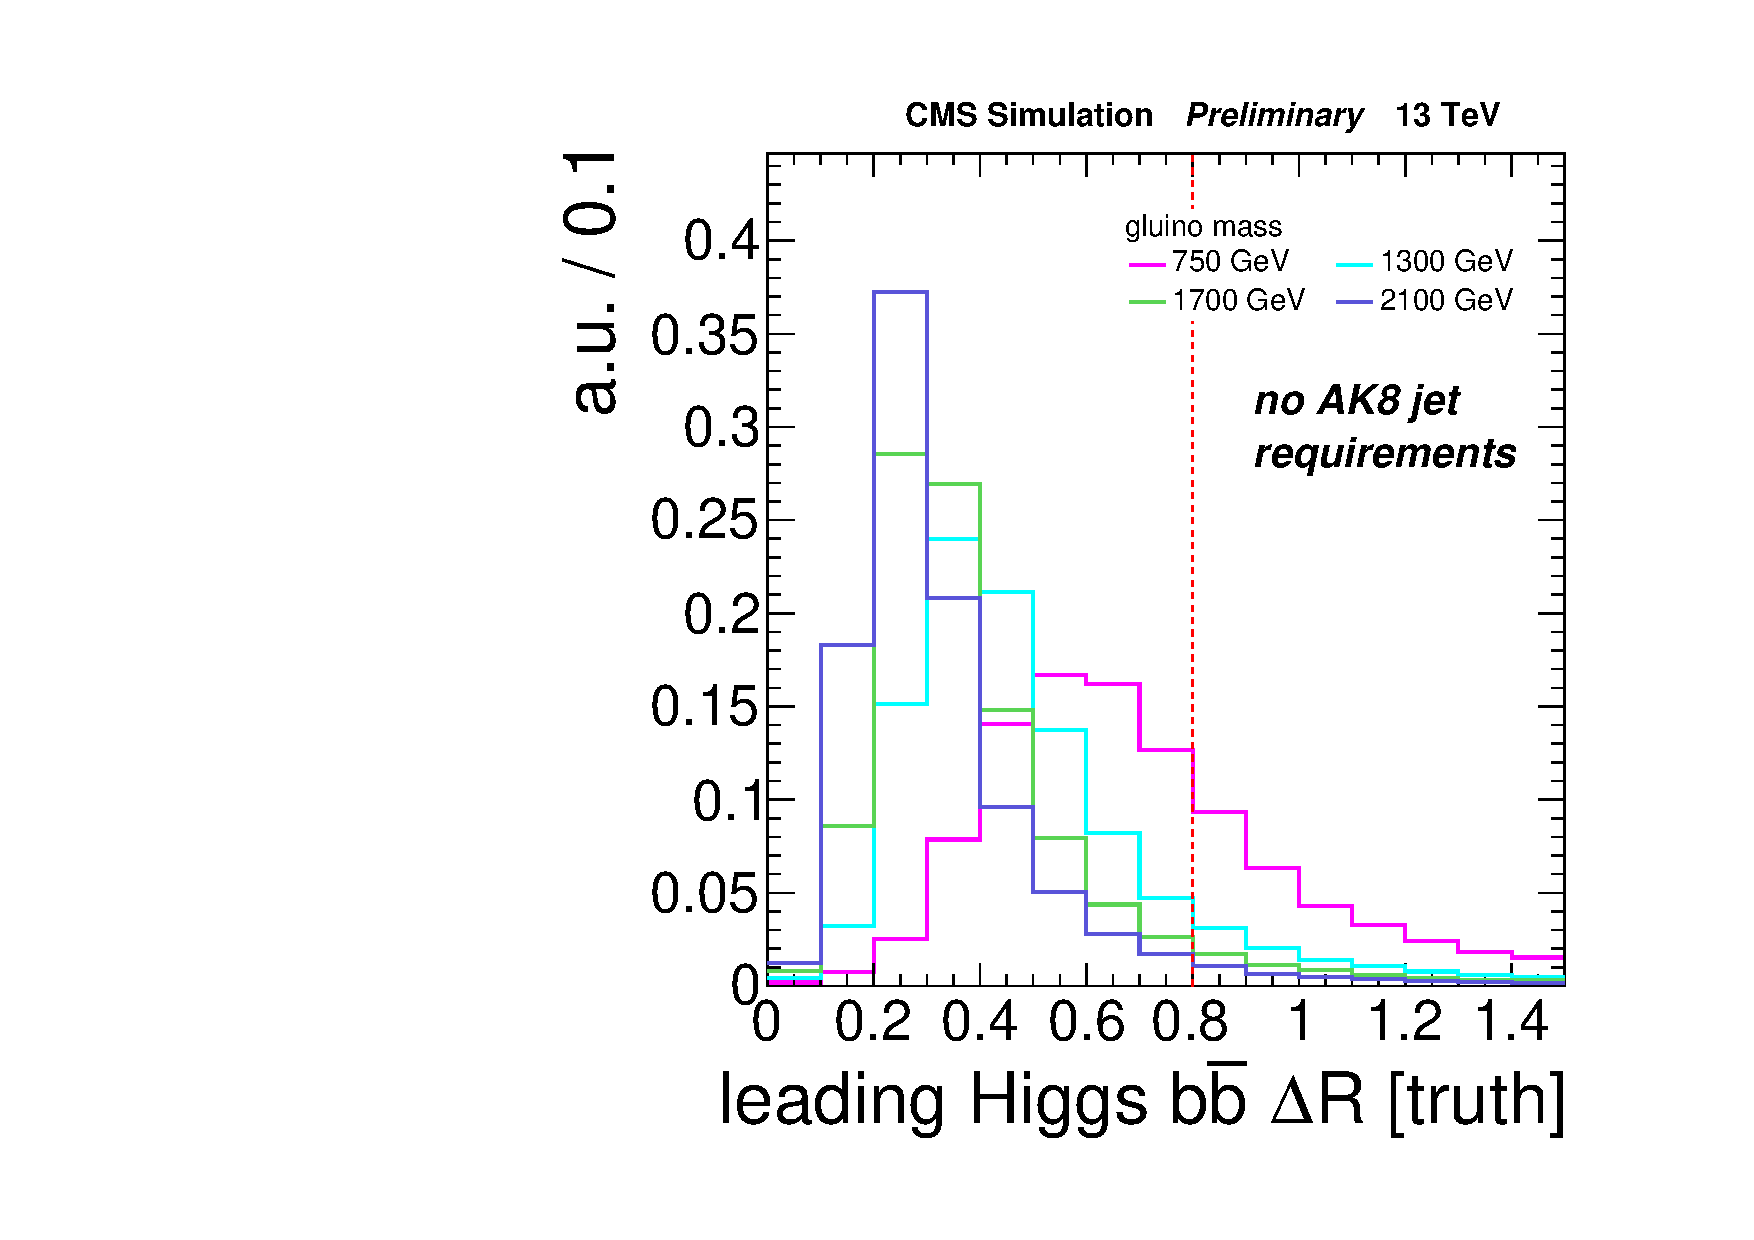
\includegraphics[width=0.45\linewidth]{figs/SUS17006/leadHiggsDr.pdf}\\
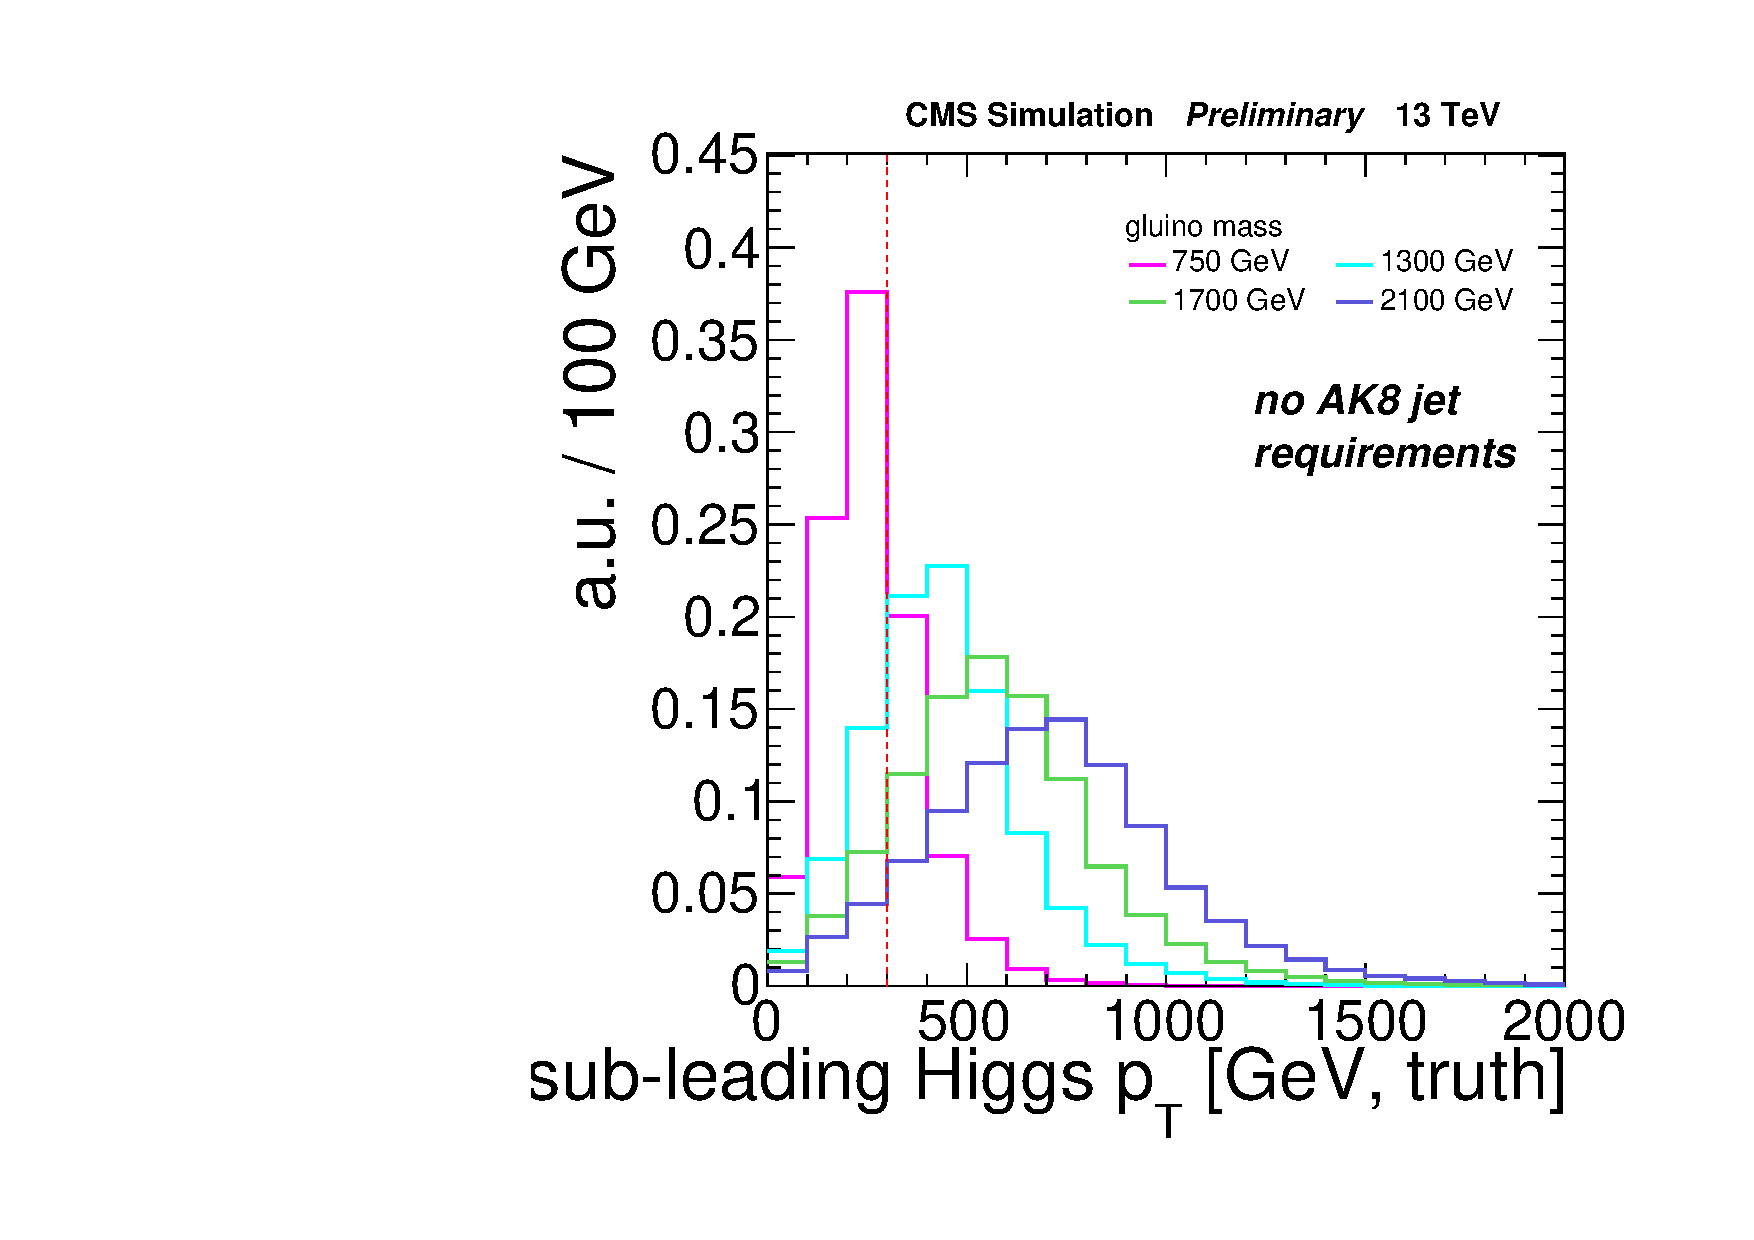
\includegraphics[width=0.45\linewidth]{figs/SUS17006/subleadHiggsPt.pdf}
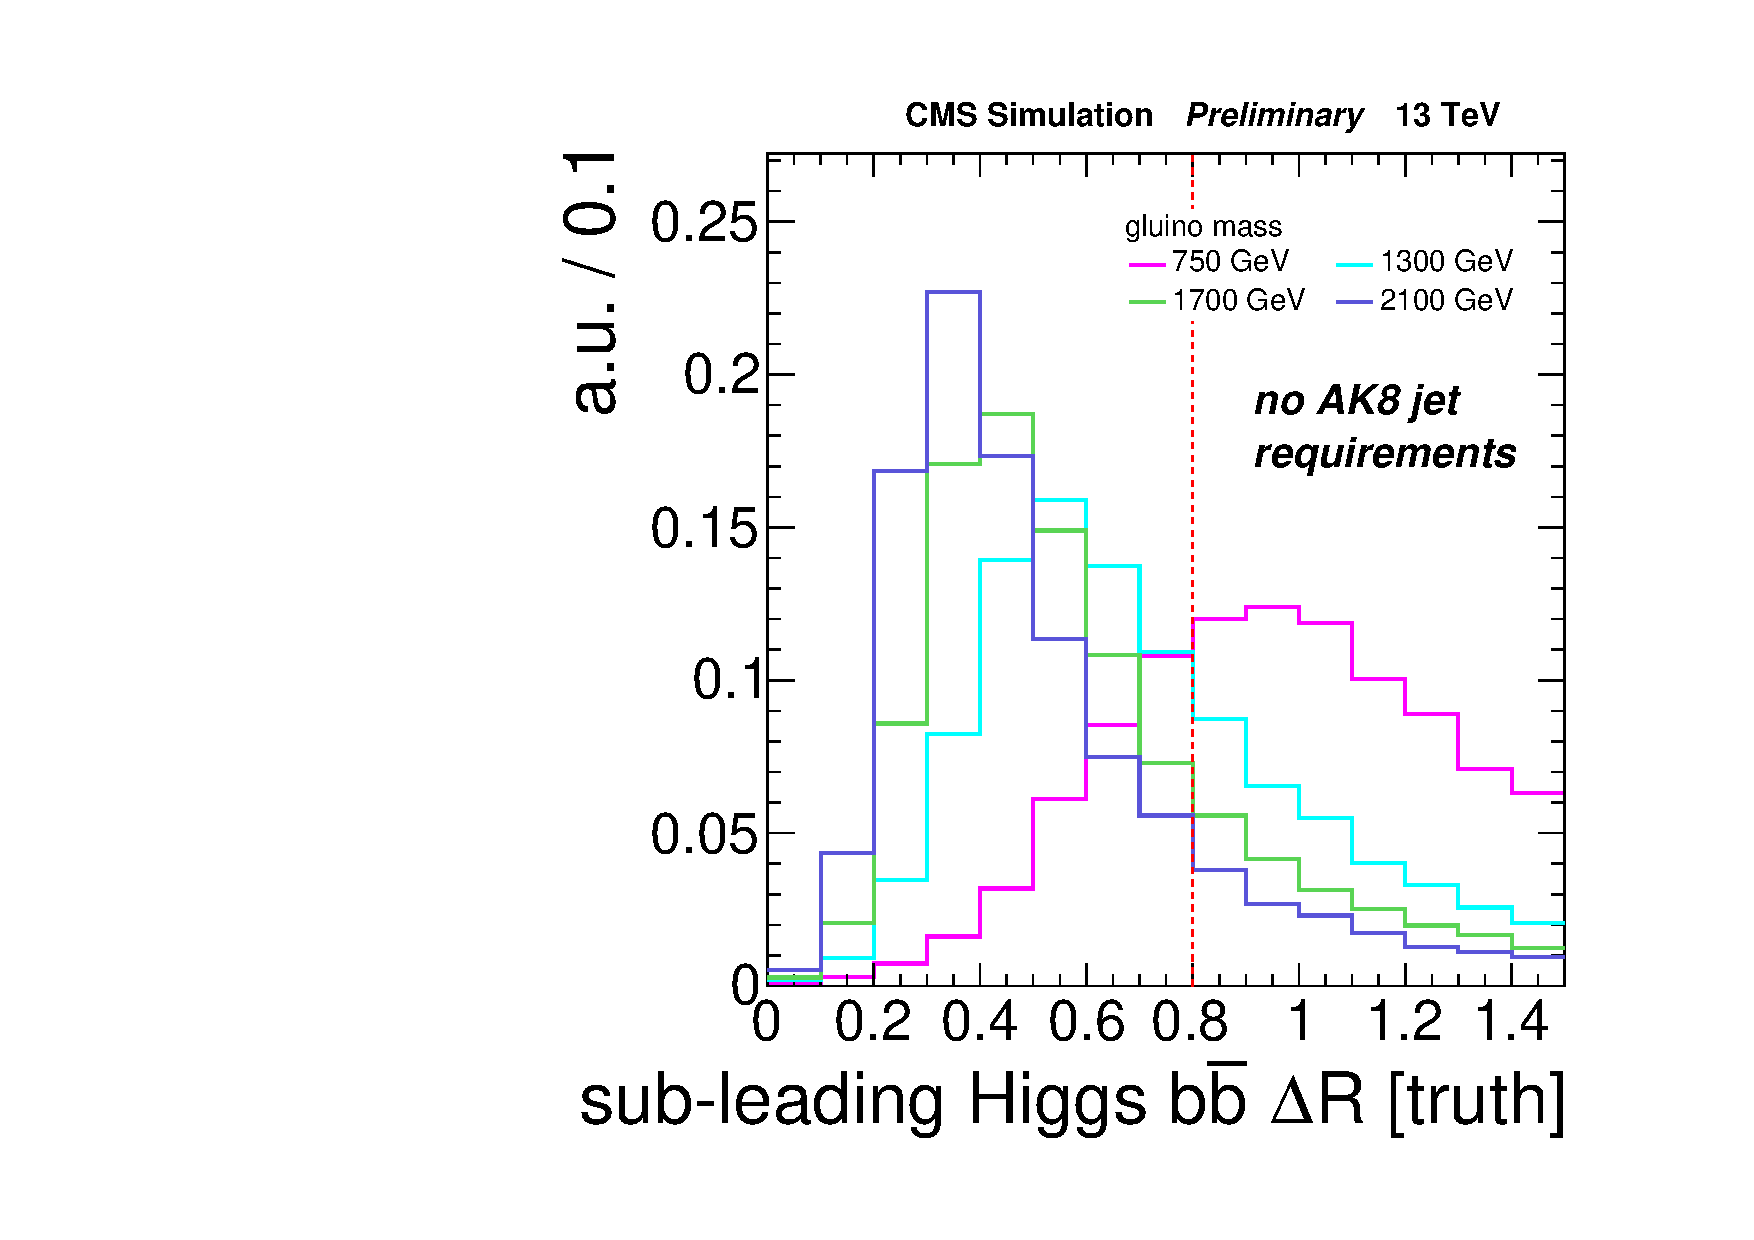
\includegraphics[width=0.45\linewidth]{figs/SUS17006/subleadHiggsDr.pdf}\\
\caption{
Generator level distributions for the leading (top row) and subleading (bottom row) H boson in the T5HH model. The plot on the left shows the $p_{T}$ of the H boson. The plot on right shows $\Delta R$ between the b-quark daughters - for large Higgs $p_{T}$ the daughters become collimated.
}
\label{fig:GenHiggsBoost}
\end{figure}

Figure \ref{fig:sms} shows the signal diagrams for the interpretations considered in this analysis. The mass splitting between the gluino $\tilde{g}$ and NLSP is fixed to 50 GeV, resulting in low $p_{T}$ quarks produced in gluino $\tilde{g}$ decays, and the mass of the LSP is fixed to 1 GeV so that the H $p_{T}$ is proportional to $m_{NLSP}/2 \sim m_{\tilde{g}}/2$. The signal regions for this analysis are designed to be sensitive to events with 2 H bosons in the final state with $H \rightarrow b\bar{b}$ or a mixed state of H and Z in the final state with an arbitrary relative branching fraction. Figure \ref{fig:GenHiggsBoost} shows the H $p_{T}$ for various $m_{\tilde{g}}$ model points. For most gluino masses, the b-quarks from $H \rightarrow b\bar{b}$ and $Z \rightarrow b\bar{b}$ are expected to be contained in a large-radius jet of $\Delta R=0.8$. Events are generated with the Full Simulation using the reconstruction in CMSSW version \texttt{8\_0\_X}.
